 %!TEX root = TFG.tex

\chapter{Development}\label{development}

    The project consists of the development of two isolated systems which interacts with each other. The first system called Cloud Analysis has as input images of a stereo camera and its associated semantic image and as output information of center of mass and objects size in the image - street, house, car, tree, sky, sidewalk and unidentified empty spaces. It was decided to consider only the case scenario with one object of each category of the semantic image in the scene, because it is still not possible to distinguish between two objects of the same category. 

    The second system receives as input the values of the center of mass and size obtained by the first system and then generates a 3D environment of its own with all objects captured by the stereo camera. It uses the Entity Component System approach for its architecture and its implementation is in the C++ language using OpenGL graphics framework.
    
    A representation of the whole system is shown in \autoref{fig:flow-system}, representing both point cloud analysis and 3D environment creation.
    
    \begin{figure}[H]
        \caption{
        \label{fig:flow-system}
            Flow representing the entire system
        }
        \begin{center}
        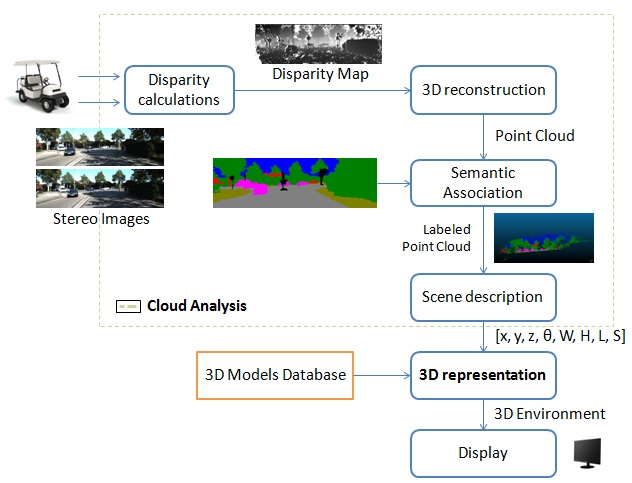
\includegraphics[width=1\textwidth]{images/fluxo1.png}
        \end{center}
        \legend{Source: Authors of this study.}
    \end{figure}    

\section{Cloud Analysis}

    Cloud Analysis is the system capable of generating a number of points which discriminates all categories of the semantic image and calculates their respective center of mass and sizes.
    
    A simple example is to imagine a real urban environment with trees, cars, houses and others. Cloud Analysis has the function of analyzing this scenario and returning the mass center value and size of each of these elements (tree, car and others). It has as output a data tuple of each element, containing: coordinates in the 3D plane of its center of mass, Width, Height, Length and a descriptor that informs which category this element is inserted.

    This system has well-defined steps: disparity image generation, point cloud generation, colored point cloud generation, and center of mass \& size calculation.
    
    For a qualitative analysis, some different tests were performed and each partial flow result can be visualized in the following topics.
    
\subsection{Disparity Calculations}

    The first part of the Cloud Analysis system is the treatment of the two input images for the disparity calculation, as shown in \autoref{fig:disparityCalFlow}. This treatment was performed as follows: The camera calibration data was provided by KITTI dataset and the Sum of Squared Differences(SSD) calculation was used in order to discover the disparity value of each pixel.

    \begin{figure}[H]
        \caption{
        \label{fig:disparityCalFlow}
            Disparity calculation flow}
        \begin{center}
        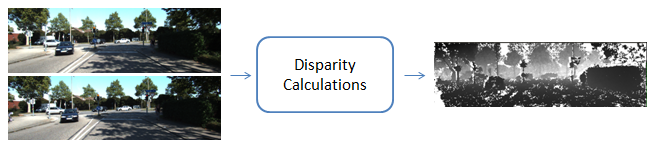
\includegraphics[width=1\textwidth]{images/disparityCalFlow.png}
        \end{center}
        \legend{Source: Authors of this study.}
    \end{figure}
    
    With camera calibration data, it is possible to define the positioning of each of the cameras and to align two images so that the already explained pixel assimilation is possible. The \autoref{Teste1-2results} and \autoref{teste3-4result} show the results obtained in four different scenario tests.

\begin{figure}[H]
  \centering
  \caption{
    The first (left) and second (right) tests and results obtained for disparity image generation. The first three images of each column are inputs (the left and right cameras and the semantic image, respectively \cite{giovaniThesis}). The latter is an image of disparity generated.}
  \label{Teste1-2results}
  \mbox{%
    \subfigure{\label{teste1a}%
      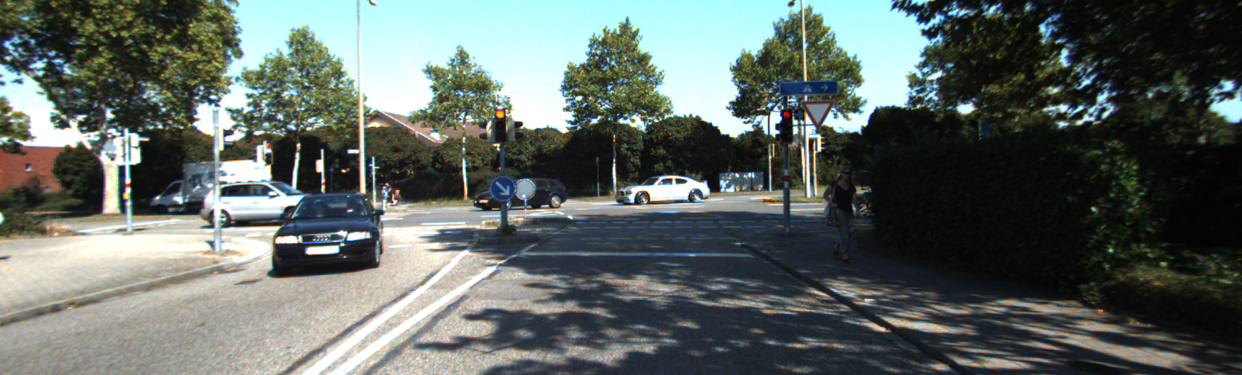
\includegraphics[width=0.4\textwidth]{images/right2.png}}\qquad
    \subfigure{\label{teste2a}%
      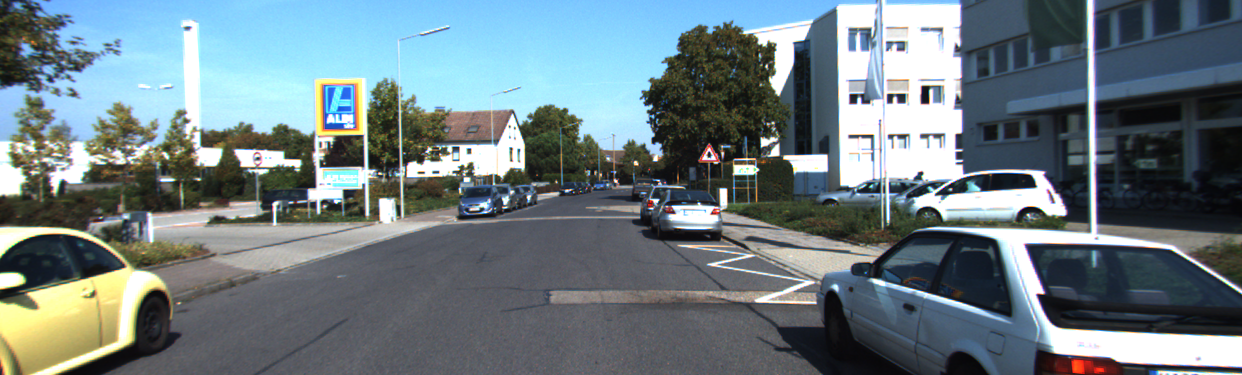
\includegraphics[width=0.4\textwidth]{images/right240.png}}
    }
    \mbox{%
    \subfigure{\label{teste1b}%
      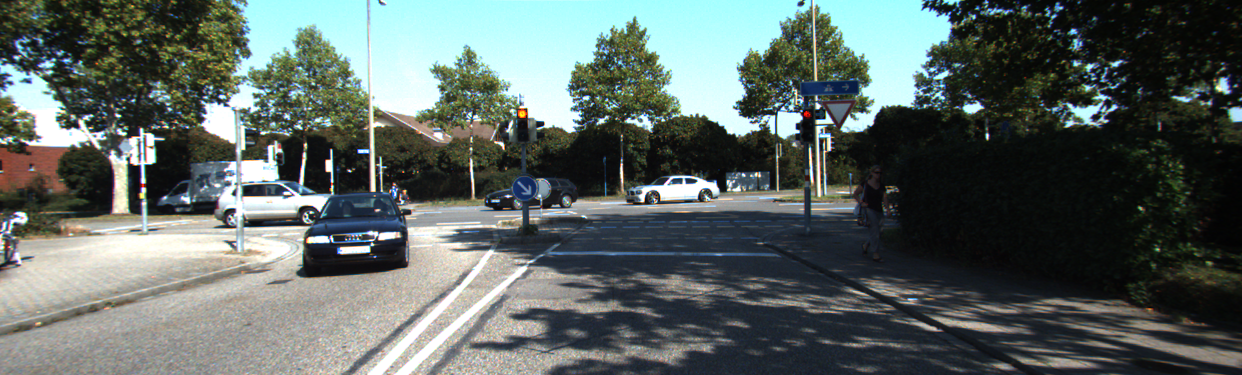
\includegraphics[width=0.4\textwidth]{images/left2.png}}\qquad
    \subfigure{\label{teste2b}%
      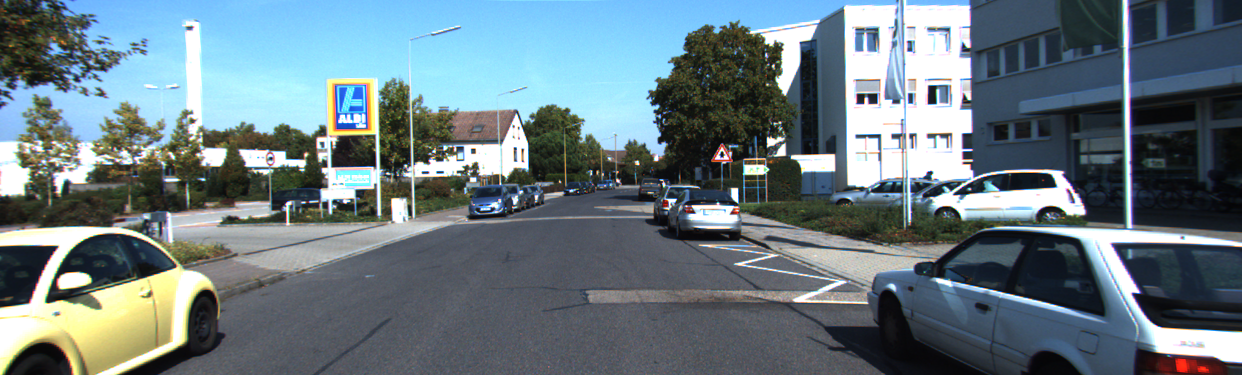
\includegraphics[width=0.4\textwidth]{images/left240.png}}
    }
    \mbox{%
    \subfigure{\label{teste1c}%
      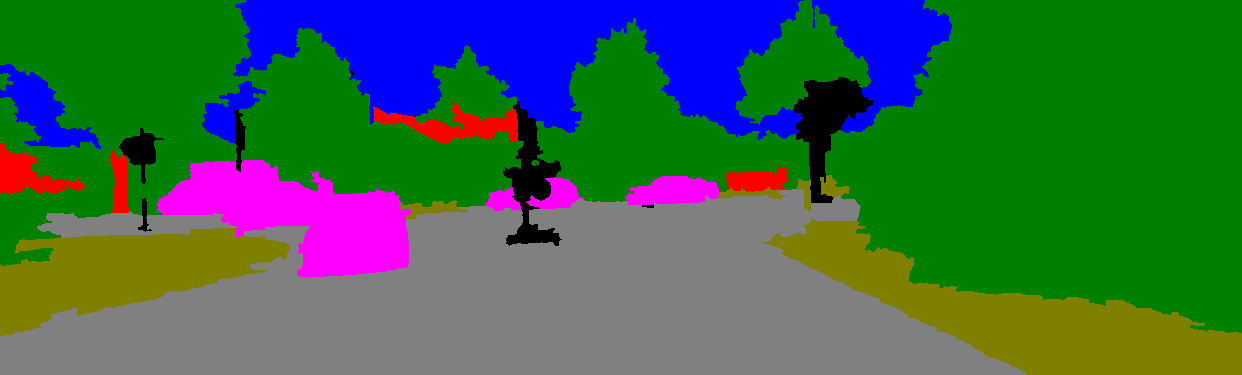
\includegraphics[width=0.4\textwidth]{images/semantica.png}}\qquad
    \subfigure{\label{teste2c}%
      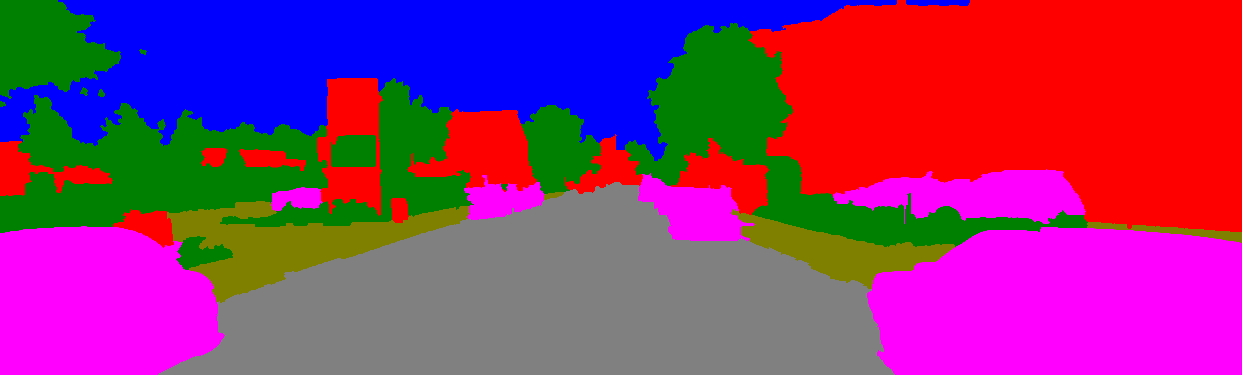
\includegraphics[width=0.4\textwidth]{images/sem240.png}}
    }
    \mbox{%
    \subfigure{\label{teste1d}%
      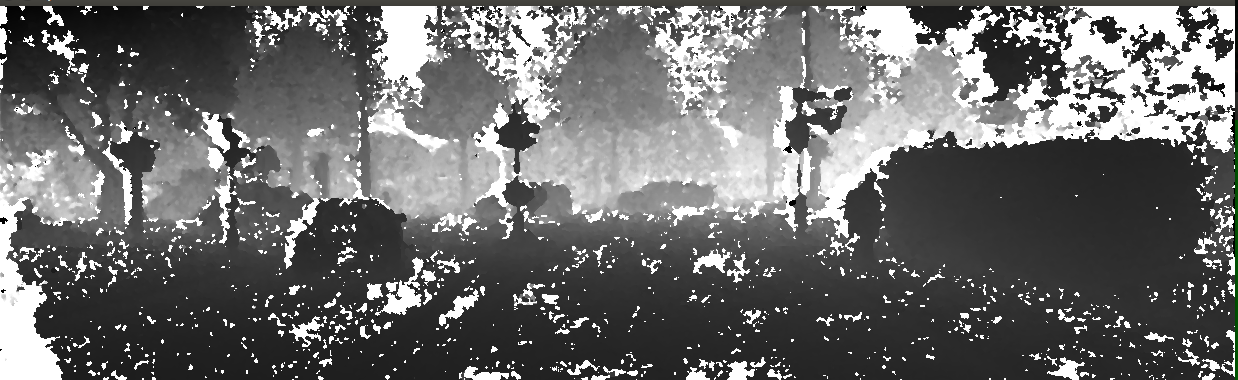
\includegraphics[width=0.4\textwidth]{images/disparity_image.png}}\qquad
    \subfigure{\label{teste2d}%
      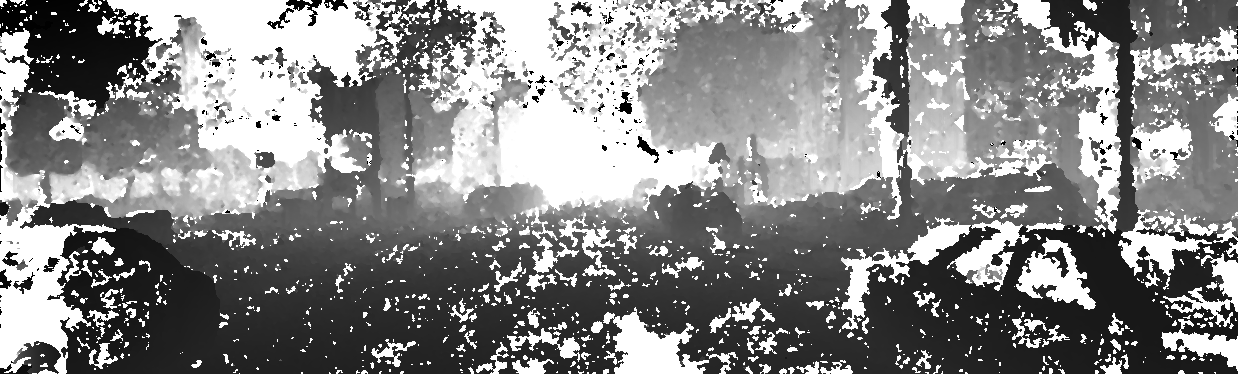
\includegraphics[width=0.4\textwidth]{images/disp240.png}}
    }
    \legend{Source: Authors of this study.}
\end{figure}

\begin{figure}[H]
  \centering
    \caption{
    The third and fourth tests and results obtained for a disparate image generation. The first three images are the system inputs (the left and right cameras and the semantic image, respectively \cite{giovaniThesis}). The latter is an image of disparity generated.
    }
  \mbox{%
    \subfigure{\label{teste3a}%
      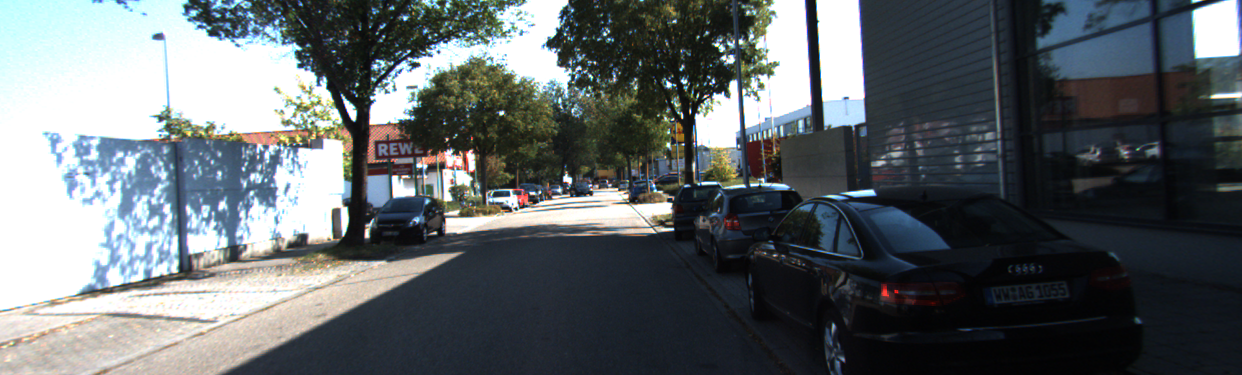
\includegraphics[width=0.4\textwidth]{images/right000.png}}\qquad
    \subfigure{\label{teste4a}%
      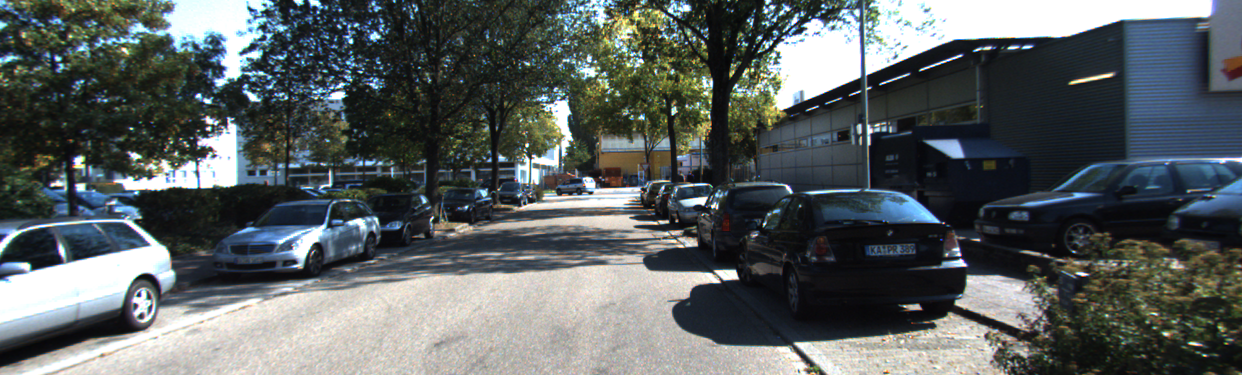
\includegraphics[width=0.4\textwidth]{images/right110.png}}
    }
    \mbox{%
    \subfigure{\label{teste3b}%
      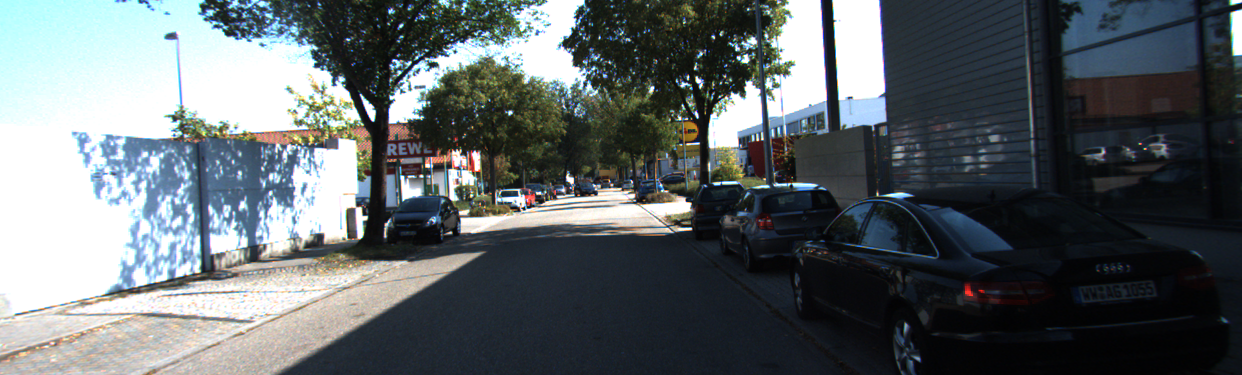
\includegraphics[width=0.4\textwidth]{images/left000.png}}\qquad
    \subfigure{\label{teste4b}%
      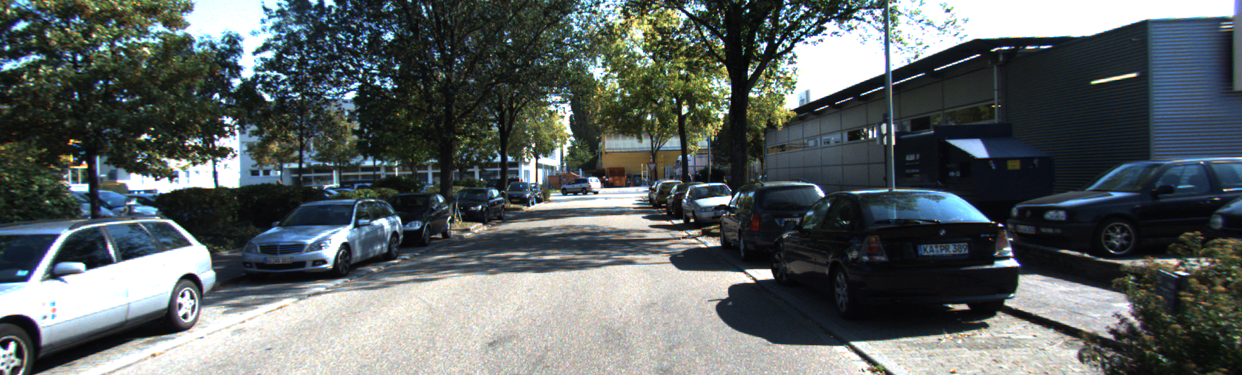
\includegraphics[width=0.4\textwidth]{images/left110.png}}
    }
    \mbox{%
    \subfigure{\label{teste3c}%
      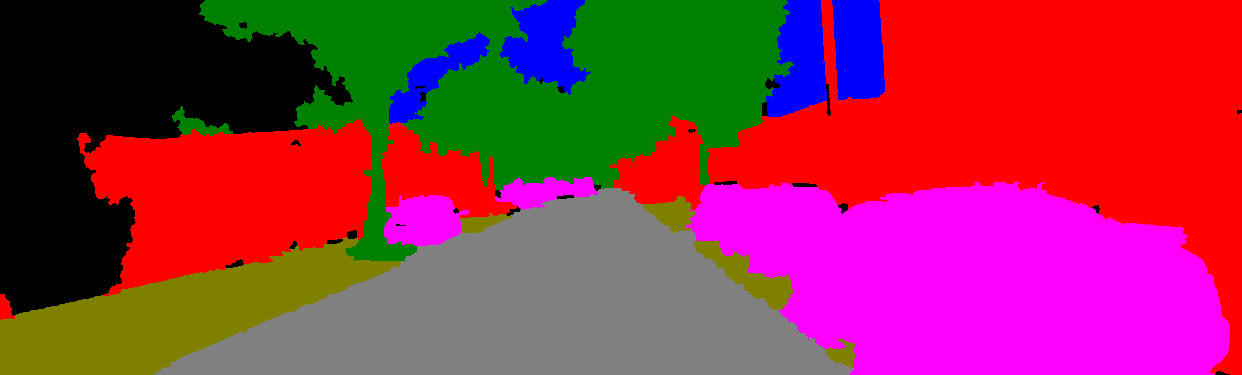
\includegraphics[width=0.4\textwidth]{images/sem000.png}}\qquad
    \subfigure{\label{teste4c}%
      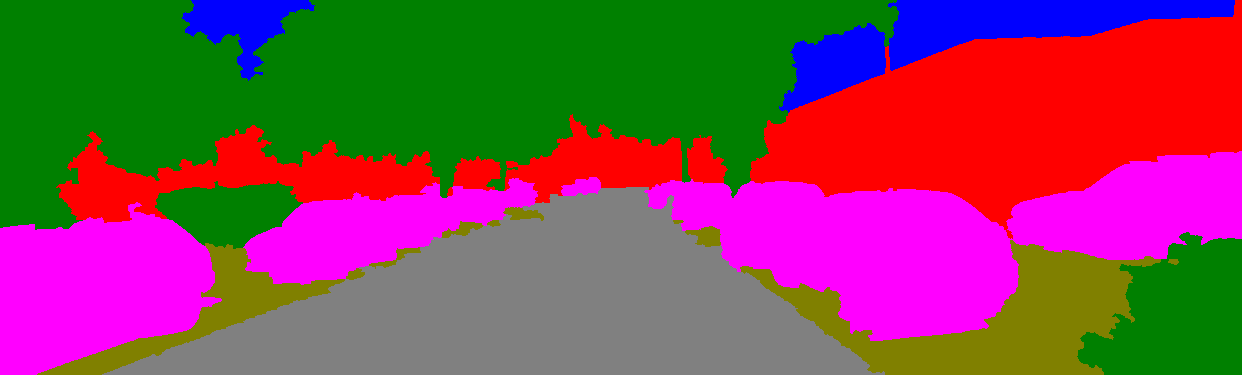
\includegraphics[width=0.4\textwidth]{images/sem110.png}}
    }
    \mbox{%
    \subfigure{\label{teste3d}%
      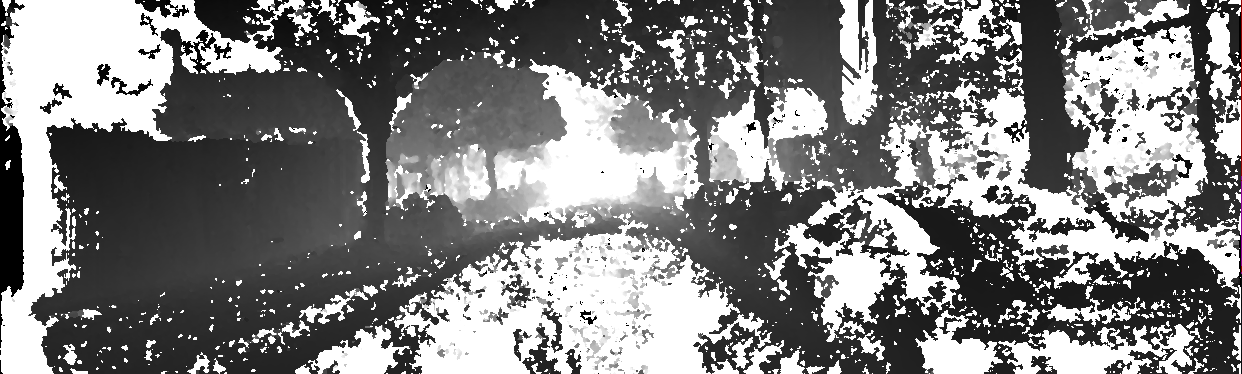
\includegraphics[width=0.4\textwidth]{images/disp000.png}}\qquad
    \subfigure{\label{teste3d}%
      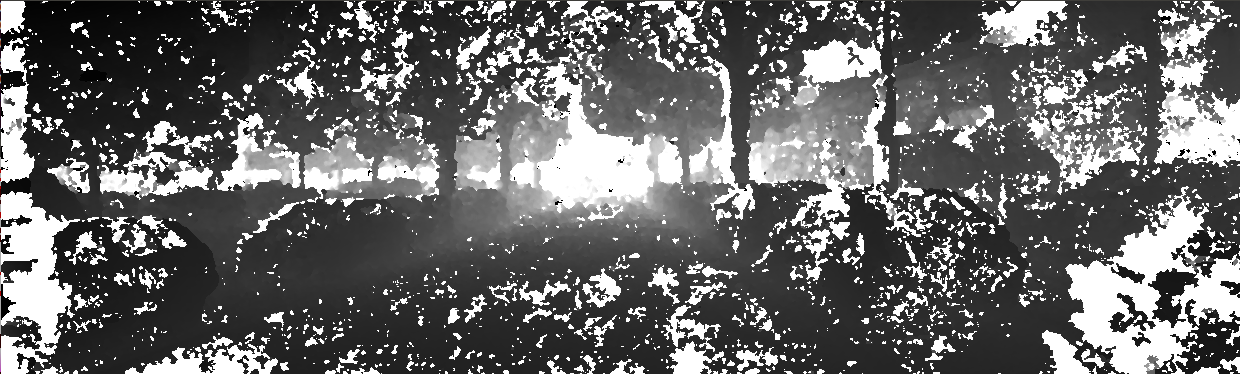
\includegraphics[width=0.4\textwidth]{images/disp110.png}}
    }
    \legend{Source: Authors of this study.}
  \label{teste3-4result}
\end{figure}

    By analyzing the resulting disparity images, one can also perceive that there is a satisfactory proximity to reality. It is possible to perceive the depth of the elements in the images in which the grayscale shows how close or far the components that make up the image are. The third test was shown to be less effective, both in the disparity image and in the color image.
    
\subsection{3D Reconstruction}
    
    The following step in this flow is the point cloud generation, as shown in \autoref{fig:CloudFlow}. 

    \begin{figure}[H]
        \caption{
        \label{fig:CloudFlow}
            Point Cloud Generation Flow}
        \begin{center}
        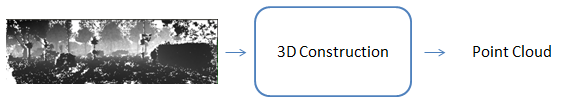
\includegraphics[width=1\textwidth]{images/CloudFlow.png}
        \end{center}
        \legend{Source: Authors of this study.}
    \end{figure}
    
    The Algorithm \autoref{pointCloudAlgo} contains the brief about the whole system developed to create a point cloud. As the Algorithm shows, the result is written in a \textit{xyz} file with 3D points position. In addition to this output, the disparity image was saved so that it could be analyzed.
    
    Using this algorithm, tests were performed using images obtained from Giovani's dataset \cite{giovaniThesis} shown in \autoref{Teste1-2results} and \autoref{teste3-4result} including photos from the right and left camera, and semantic image.

\IncMargin{1em}
\begin{algorithm}
\label{pointCloudAlgo}
\SetKwData{Left}{left}\SetKwData{This}{this}\SetKwData{Up}{up}
\SetKwFunction{Union}{Union}\SetKwFunction{FindCompress}{FindCompres}
\SetKwInOut{Input}{input}\SetKwInOut{Output}{output}
\Input{ Two OpenCV's cv::Mat matrices that represent the right and left photos. In addiction, the respective semantic image of the scene.}
\Output{ A file in \textit{xyz} format that contains a set of 3D points associated to a value. This value represents the distance between the 3D point and the camera.}
\BlankLine
\emph{Camera Calibration according to data collected during camera setup}\;
\emph{Converting photos to grayscale images}\;
\emph{Setup specific values of calibration to use OpenCV's cv::StereoSGBM class}\;
\emph{Disparity image generation by the cv::StereoSGBM class with stereo images as input}\;
\emph{Normalize disparity image to 0-255 scale}\;
\emph{Create a Mat matrix called Points that store 3D points information of the cloud point from the OpenCV's cv::reprojectImageTo3D function}\;    
\For{$i\leftarrow 0$ \KwTo $points.rows$}{
\For{$j\leftarrow 0$ \KwTo $points.cols$}{\label{forins}
\emph{Writing in a \textit{xyz} file the X, Y and Z position of each point and the intensity value (grayscale) related to the distance between point and camera}\;}}
\emph{Printing the result}\;
\caption{Point Cloud Generation}\label{algo_disjdecomp}
\end{algorithm}\DecMargin{1em}

    The image of a point cloud obtained from the photos of left and right is a set of grayscale points with low visualization value as there is to differentiation of entity representation. For this reason, point cloud results were expressed only by the end, in the Colored Point Cloud that uses semantic information to define entities.
    
\subsection{Semantic Association}

    Semantic association means a approach to create a point cloud colored, as shown \autoref{fig:colorFlow}.
    
    \begin{figure}[H]
        \caption{
        \label{fig:colorFlow}
            Semantic Association Flow}
        \begin{center}
        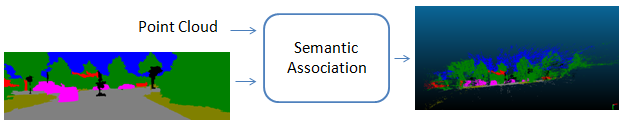
\includegraphics[width=1\textwidth]{images/colorFlow.png}
        \end{center}
        \legend{Source: Authors of this study.}
    \end{figure}
    
    The following steps occurred from the following algorithm: Reading the whole Point Cloud xyz file generated in Algorithm \autoref{pointCloudAlgo}; Reading the semantic image and record the respective RGB (Red, Green and Blue) values to each pixel of the image; Gathering the two values into a single file that contains the following attributes in each row: x, y, and z position of the pixel, its grayscale value and its RGB values.

    There is a program called Cloud Compare that reads \textit{xyz} files and shows the point cloud with color and interact with them. Using this program we were able to display the results shown in \autoref{testeColoredCloud}.

    In \autoref{testeColoredCloud}, each image represents the result of a test, first picture represents first test and the numeration goes top-down. The first test proved to be the most efficient of all which showed a wealth of detail in both near and camera and distant images. The second and fourth tests were also close to reality, especially near the camera.

    The worst test generated was the third test. In this test, the disparity image generated and its point cloud interpreted much of the street as something below the ground, as shown in \autoref{testeColoredCloud} (gray pixels filling the subsoil). It seems that it is related to the fact that the section with few details is very dark, which leads to difficulties in the generation of the disparity image. In addition, it is noted that the semantic image for this photo interpreted as void space much of the sky on the left.
    
\begin{figure}[H]
  \centering
    \caption{
    Colored Point Cloud results}
    \subfigure{\label{testeColor1}%
      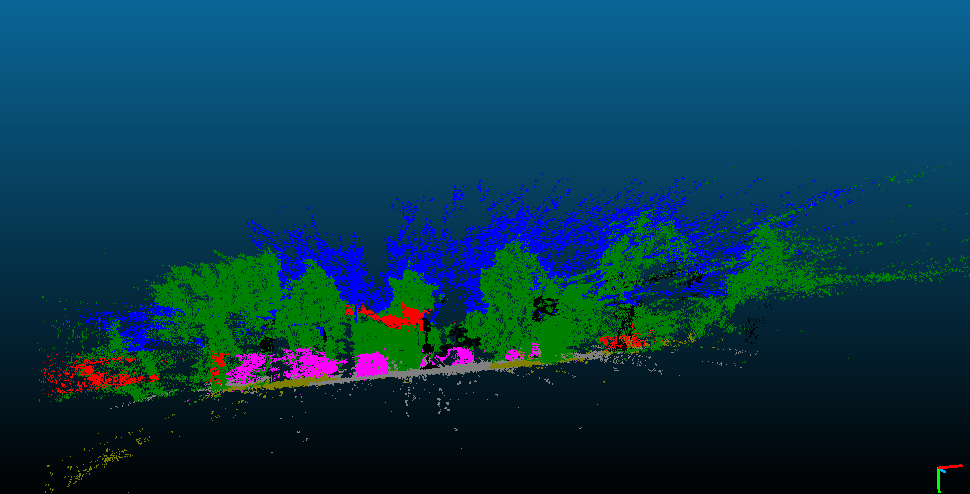
\includegraphics[width=0.6\textwidth]{images/color2.png}}\qquad
    \subfigure{\label{testeColor2}%
      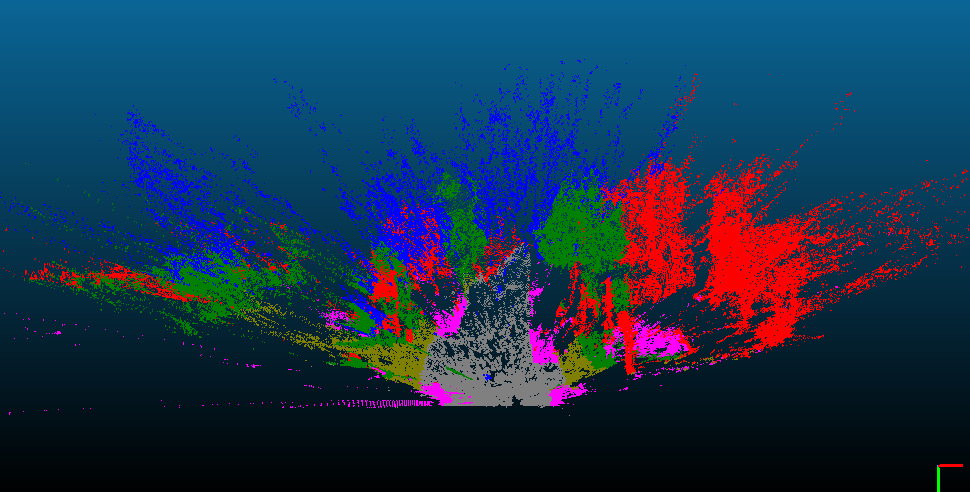
\includegraphics[width=0.6\textwidth]{images/color240(2).png}}\qquad
    \subfigure{\label{testeColor3}%
      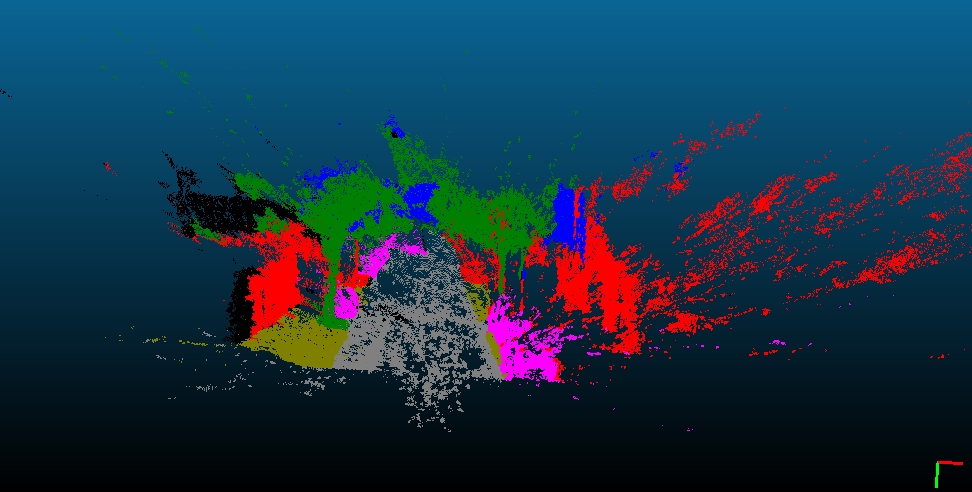
\includegraphics[width=0.6\textwidth]{images/color000(2).png}}\qquad
    \subfigure{\label{testeColor4}%
      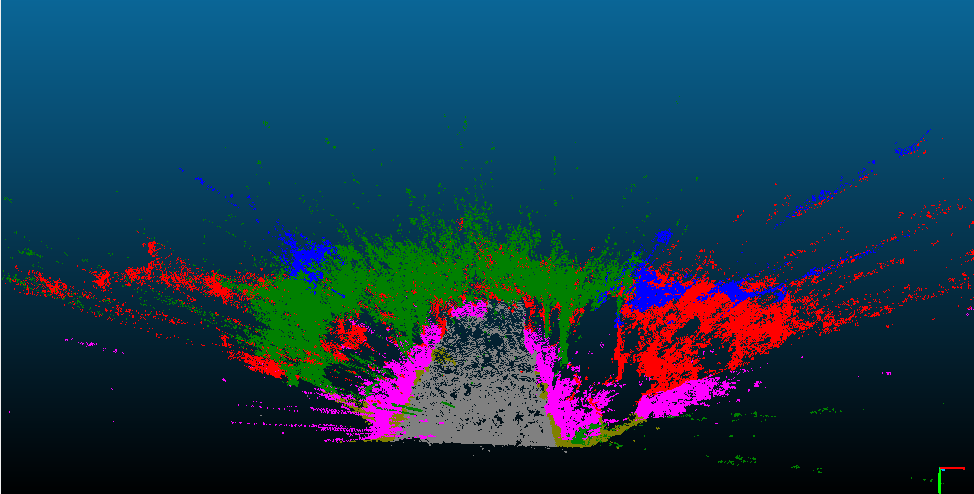
\includegraphics[width=0.6\textwidth]{images/color110(2).png}}
    \legend{Source: Authors of this study.}
  \label{testeColoredCloud}
\end{figure}    

    
\subsection{Scene Description}

    After the 3D coordinate data and colors have been acquired in the algorithm to obtain the colored point cloud, it is necessary to discriminate the categories and calculate the center of mass and size of each one of them. The flow to do this is represented in \autoref{fig:SceneFlow}. Note that x, y and z represent the x, y, and z coordinates of the center of mass; Theta is the direction of the object in the 3D scenario; W, H and L are the width, height and length that will define the space that the object occupies and S represents what kind of object it is (such as house, vehicle, street and others).
    
    \begin{figure}[H]
        \caption{
        \label{fig:SceneFlow}
            Scene Description Flow}
        \begin{center}
        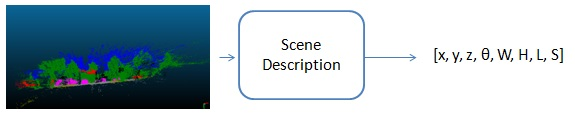
\includegraphics[width=1\textwidth]{images/sceneFlow.png}
        \end{center}
        \legend{Source: Authors of this study.}
    \end{figure}    
    
    The project is still not able to discriminate a car from another car in the same scene, or a tree from another. Thus, it was decided that the system would assume that there would be only one possible entity: one car, one tree, one building and so on. After the system is able to operate under these conditions it would proceed to a more advanced stage of distinguishing objects within the same category.

    Before calculating the center of mass and the size of the categories contained in the scene, it was necessary to separate them. Thus, an algorithm was developed to read the \textit{xyz} file of the colored point cloud and to separate into a data structure each of the points with equal colors. All the pink objects were stored in a structure called a car, the blues in the structure called sky and the logic remain for the other categories that the semantic image can distinguish.

    Since the assumption is that the system has one element of each category, it is sufficient to calculate the center of mass (\autoref{eq:MassCenterX2}, \autoref{eq:MassCenterY2}, \autoref{eq:MassCenterZ2} ) of each structure separately. In the end, there are seven different center of mass values: One for car, building, tree, sky, sidewalk, street and unidentified void space.

    At this moment, only the calculation of the average of points located in the different directions in relation to the center of mass is done, forming a type of box that would delimit the object boundaries.
    
    To validate the center of mass values, some tests were performed where there is only one element of a certain category in the image. This element had its center of mass calculated and printed on Point Cloud Colored. The first test performed can be seen in \autoref{Teste1Center}. These are two different images in which there is only one car - one car in the first column and one car behind a sign in the second column. In this test it can notice the entire development flow of Cloud Analysis so far: Receiving three images as input and generating a disparity map, a Point Cloud, and output tuples with the center of mass information and size.

    \begin{figure}[H]
  \centering
  \caption{
First and second tests performed with only one car on the scene}
  \label{Teste1Center}
  \mbox{%
    \subfigure{\label{teste1a}%
      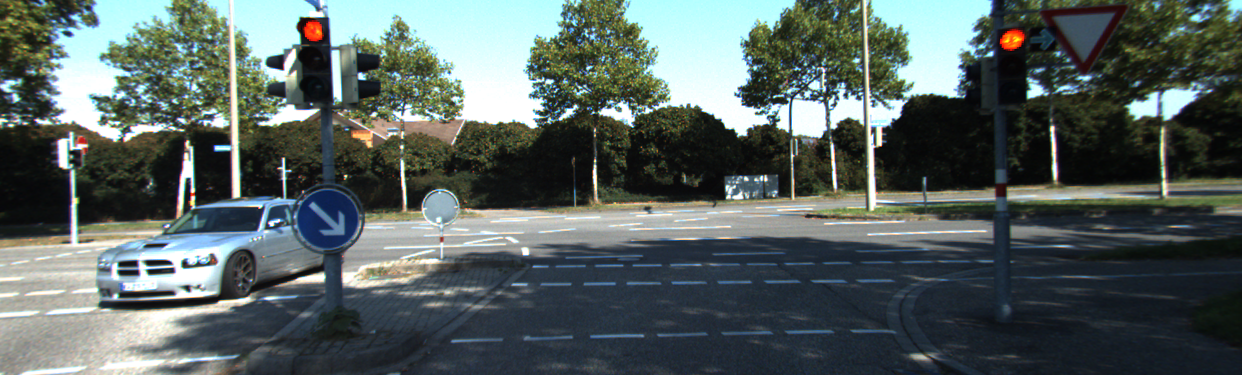
\includegraphics[width=0.4\textwidth]{images/right415.png}}\qquad
    \subfigure{\label{teste2a}%
      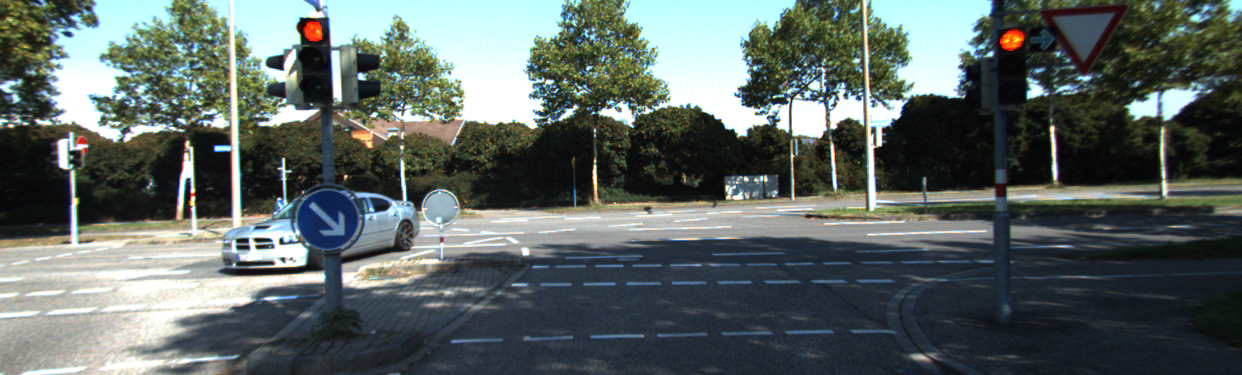
\includegraphics[width=0.4\textwidth]{images/right410.png}}
    }
    \mbox{%
    \subfigure{\label{teste1b}%
      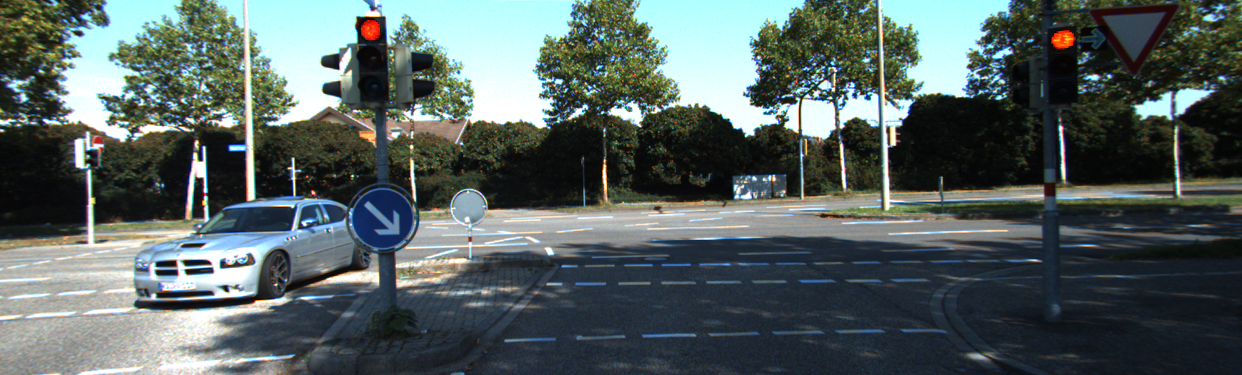
\includegraphics[width=0.4\textwidth]{images/left415.png}}\qquad
    \subfigure{\label{teste2b}%
      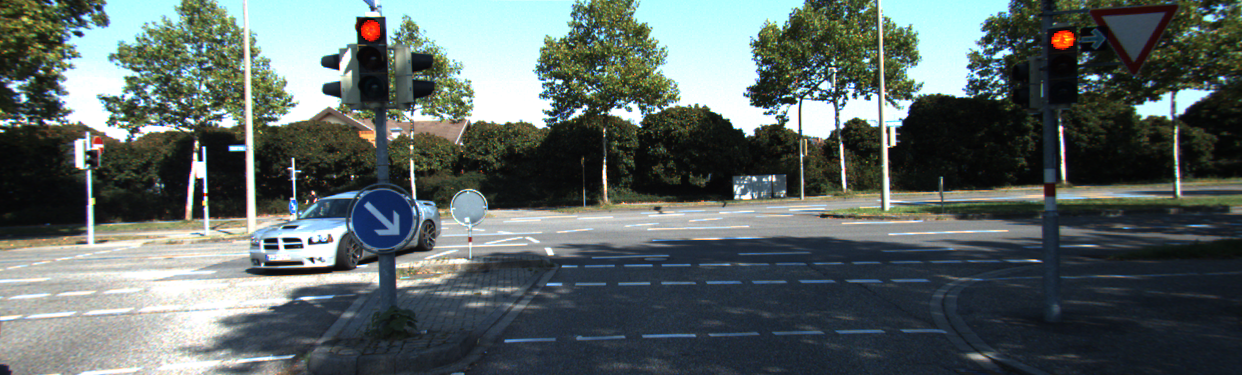
\includegraphics[width=0.4\textwidth]{images/left410.png}}
    }
    \mbox{%
    \subfigure{\label{teste1c}%
      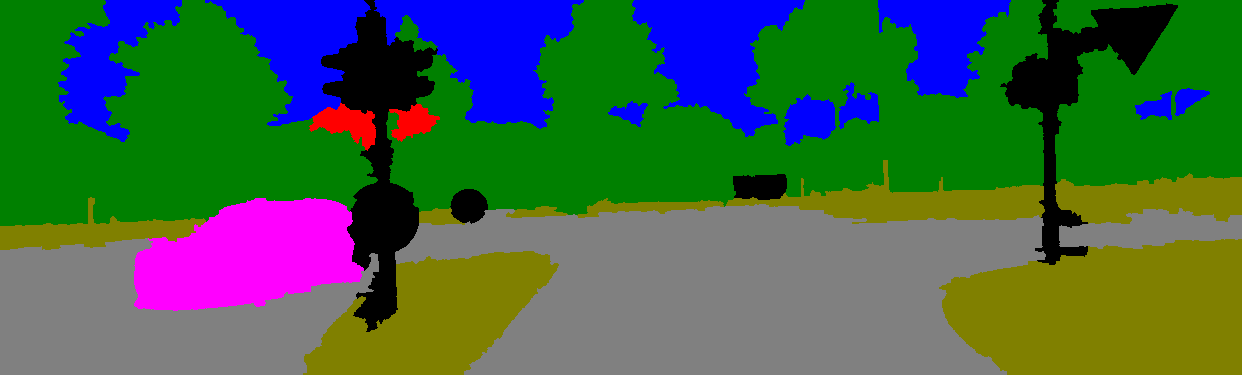
\includegraphics[width=0.4\textwidth]{images/sem415.png}}\qquad
    \subfigure{\label{teste2c}%
      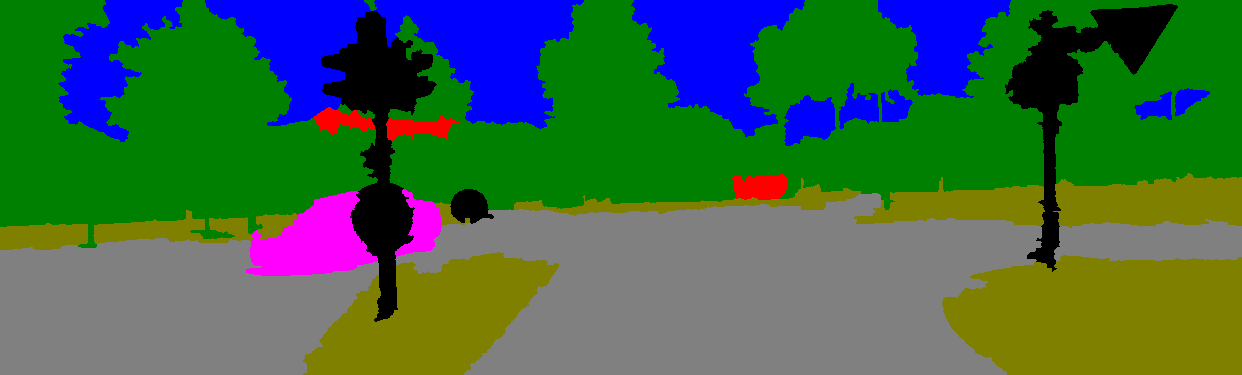
\includegraphics[width=0.4\textwidth]{images/sem410.png}}
    }
    \mbox{%
    \subfigure{\label{teste1d}%
      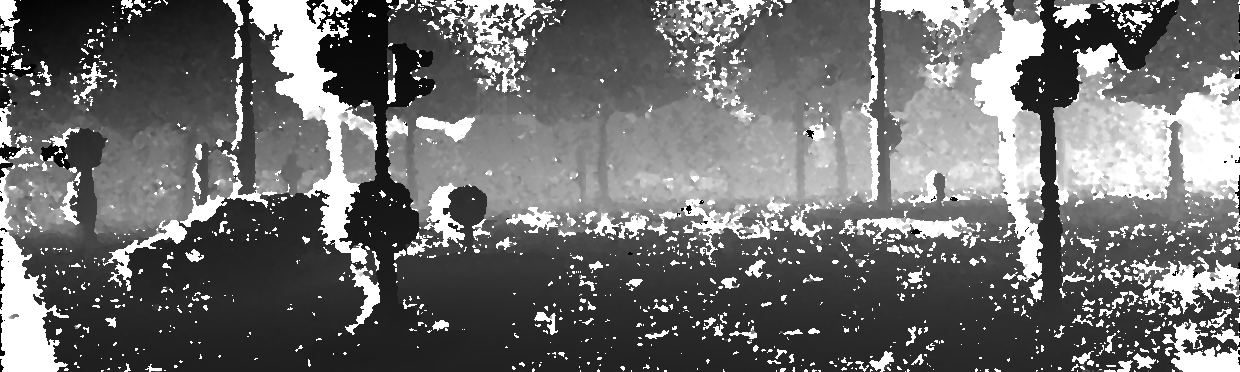
\includegraphics[width=0.4\textwidth]{images/disp415.png}}\qquad
    \subfigure{\label{teste2d}%
      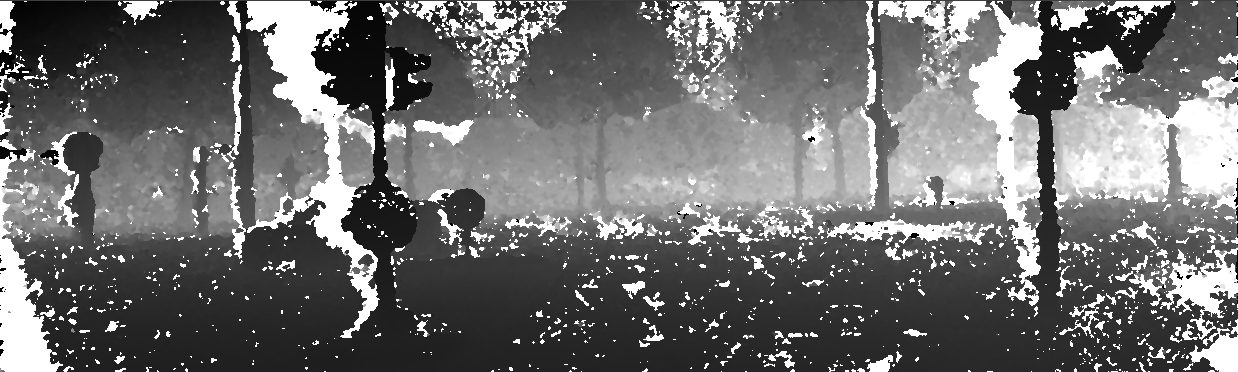
\includegraphics[width=0.4\textwidth]{images/disp410.png}}
    }
    \mbox{%
    \subfigure{\label{teste1d}%
      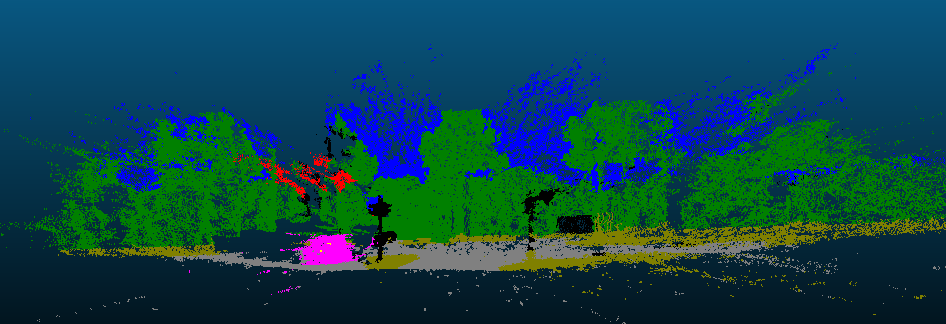
\includegraphics[width=0.4\textwidth]{images/color415.png}}\qquad
    \subfigure{\label{teste2d}%
      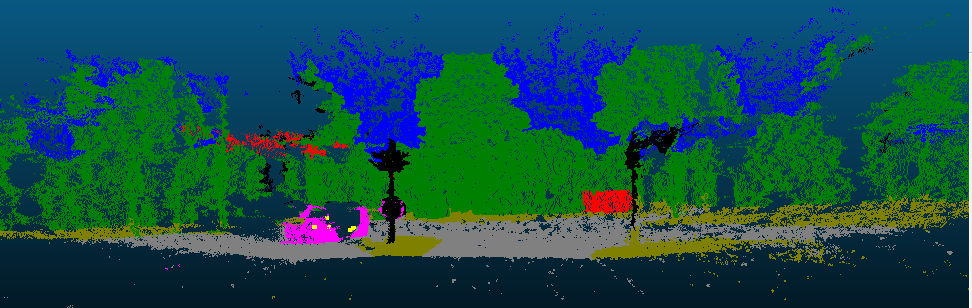
\includegraphics[width=0.4\textwidth]{images/color410.png}}
    }
    \mbox{%
    \subfigure{\label{teste1d}%
      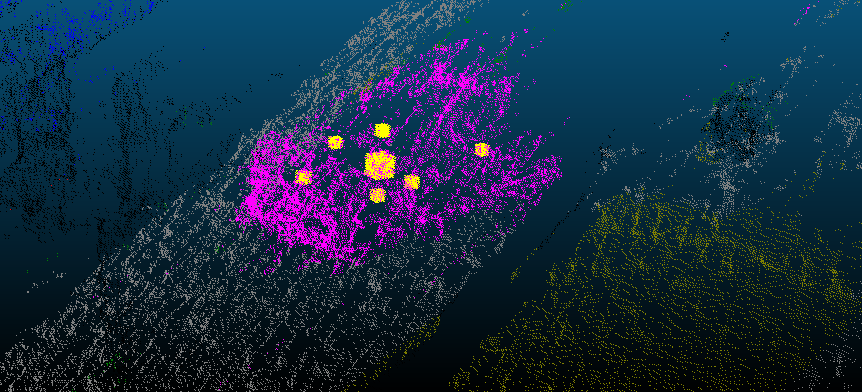
\includegraphics[width=0.4\textwidth]{images/zoom415.png}}\qquad
    \subfigure{\label{teste2d}%
      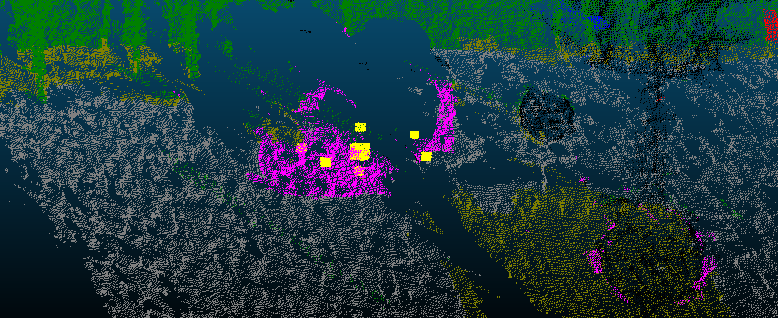
\includegraphics[width=0.4\textwidth]{images/zoom410.png}}
    }
    \legend{Source: Authors of this study.}
\end{figure}
    
    In the last image you can see that the center of mass of the car is also being printed - visually close to what would really be the center of it. On the other hand, the size limits described as small yellow squares around the center of mass were not very efficient. All points are assuming values below the actual size of the vehicle.

    It is also noted in the second column that, although the sign disrupts the complete view of the car, the center of mass values remained faithful.
    
    This test quoted above was calculated from the average points located on each of the six sides around the center of mass, as explained in the Literature Review. In order to improve the obtained results, it was decided to apply the variance method. The result and difference can be seen in \autoref{varianceRes}.

    \begin{figure}[H]
      \centering
        \caption{
        Average method vs Variance method}
        \subfigure{\label{varianceRes}%
          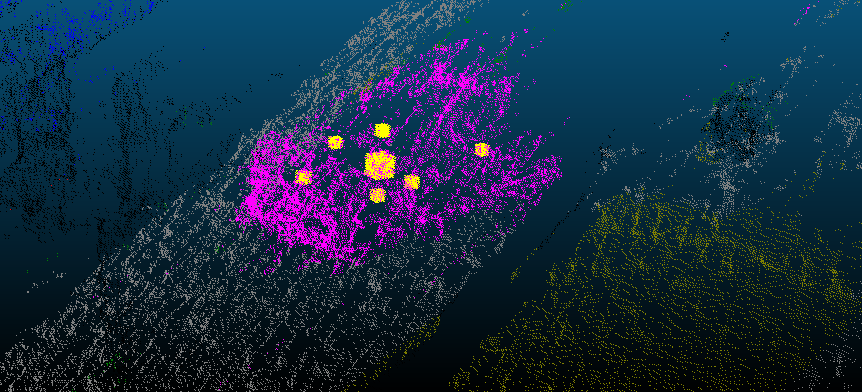
\includegraphics[width=0.6\textwidth]{images/zoom415.png}}\qquad
        \subfigure{\label{testeColor2}%
          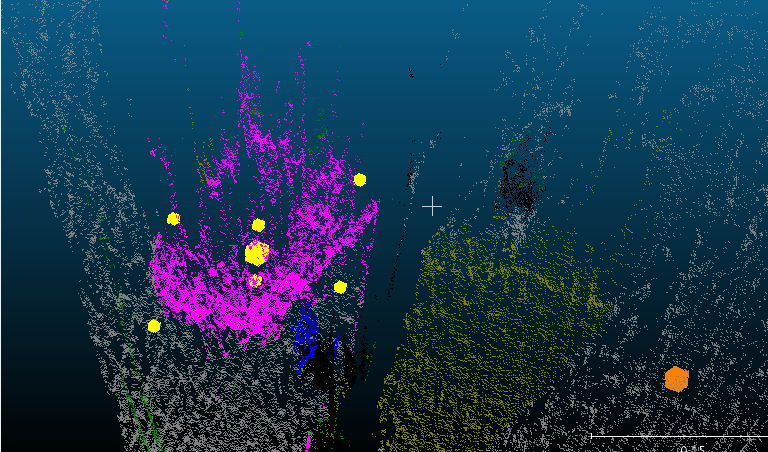
\includegraphics[width=0.6\textwidth]{images/var415.png}}\qquad
        \legend{Source: Authors of this study.}
      \label{testeColoredCloud}
    \end{figure} 
    
    It can see that the bounding box is still not perfect. Before it was too small and now, it is bigger than the real. Despite this, both results proved adequate to create a representation of the car's bounding box.It was defined to used the variance.
    
    Another test was performed considering situations where there is only one street. The function of this test is to validate the center of mass calculation of other categories besides vehicles. The street will have a different treatment in the 3D environment, however, the output of Cloud Analysis will be similar to vehicles. As shown in \autoref{Teste2Center}, the street's center of mass is located at a visually expected point, marked orange in the images.
    
    The results obtained from the center of mass (both in \autoref{Teste1Center} and in \autoref{Teste2Center}) are defined in a range of values different from the 3D environment. The functions and calculations performed for the Point Cloud generation return as a result values approximately between 5 and - 5 floating values - which is far from representing a metric close to the metric of reality.
    
    \begin{figure}[H]
  \centering
  \caption{
First and second tests performed with only one street on the scene}
  \label{Teste2Center}
  \mbox{%
    \subfigure{\label{teste1a}%
      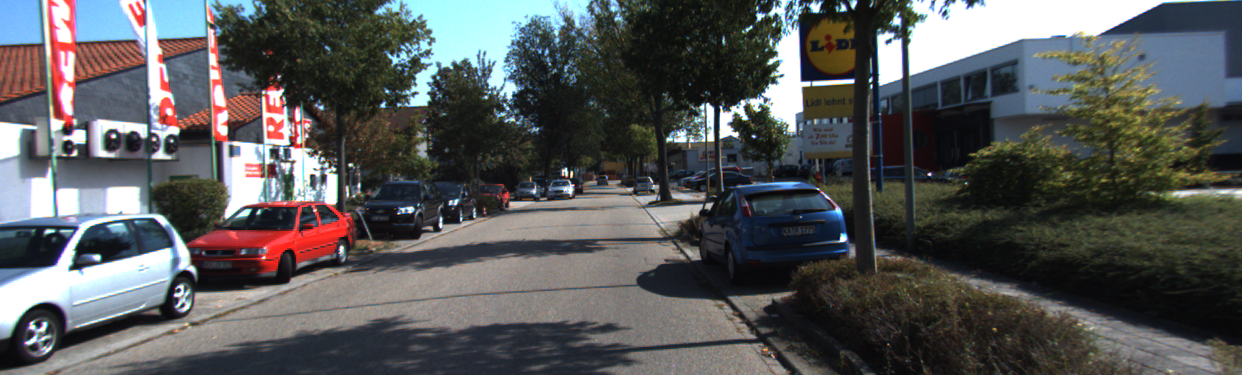
\includegraphics[width=0.4\textwidth]{images/right35.png}}\qquad
    \subfigure{\label{teste2a}%
      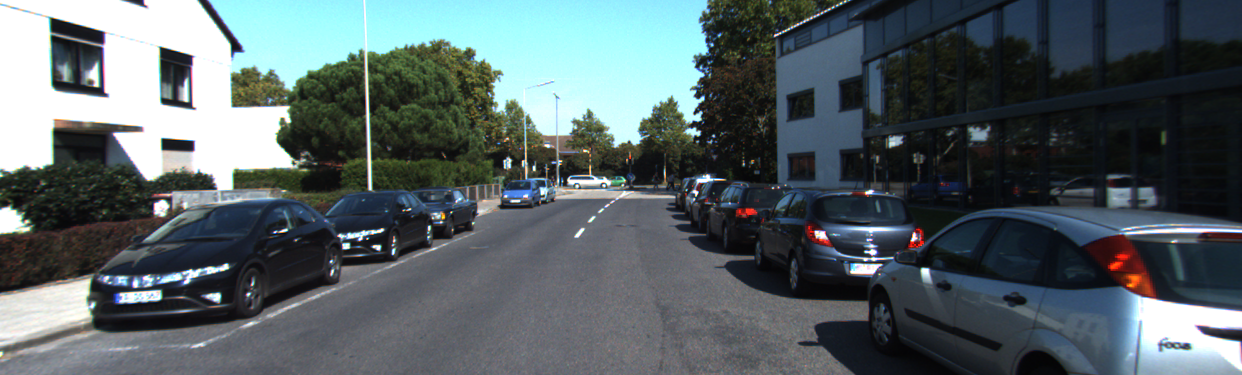
\includegraphics[width=0.4\textwidth]{images/right310.png}}
    }
    \mbox{%
    \subfigure{\label{teste1b}%
      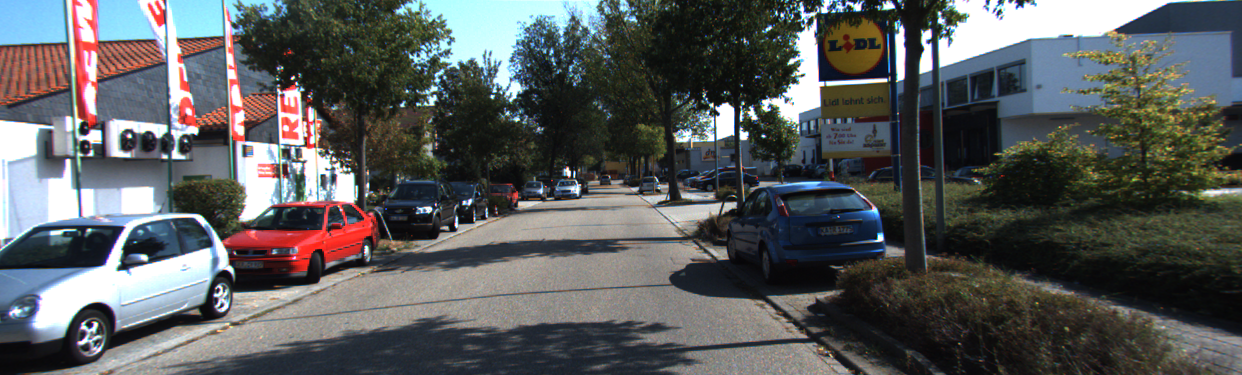
\includegraphics[width=0.4\textwidth]{images/left35.png}}\qquad
    \subfigure{\label{teste2b}%
      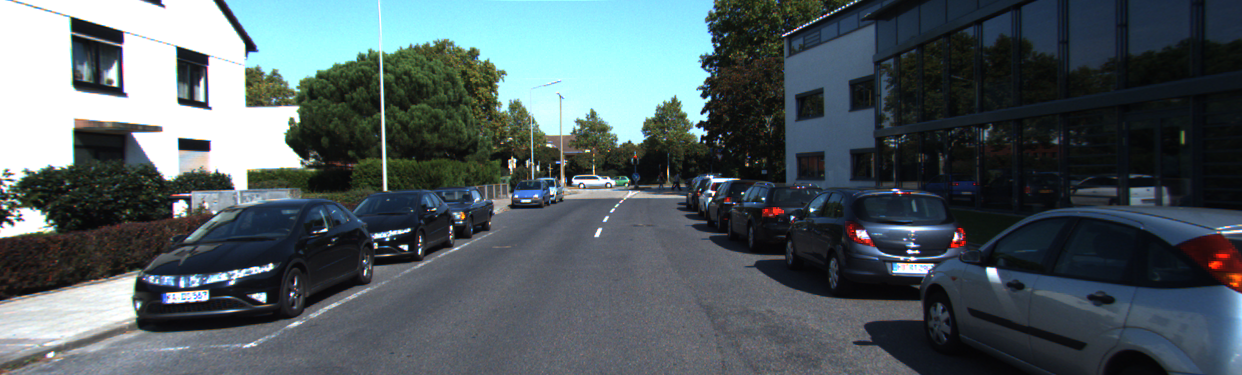
\includegraphics[width=0.4\textwidth]{images/left310.png}}
    }
    \mbox{%
    \subfigure{\label{teste1c}%
      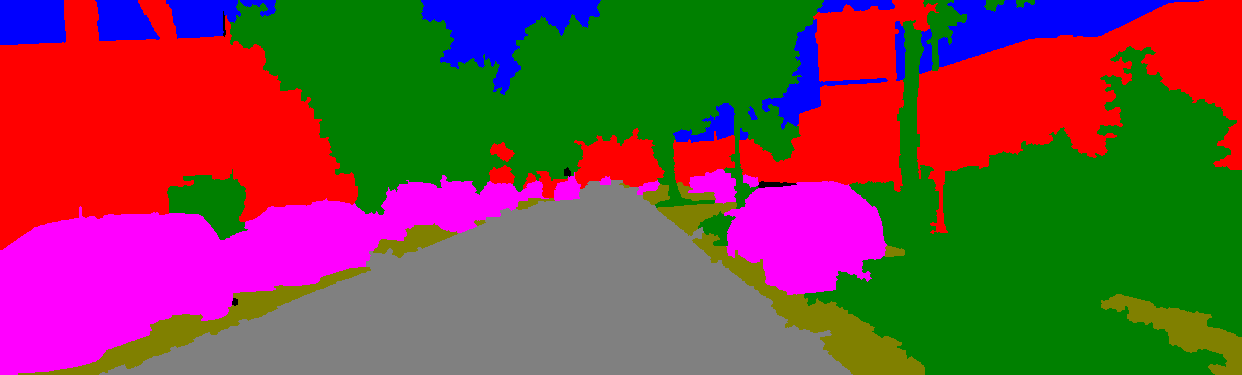
\includegraphics[width=0.4\textwidth]{images/sem35.png}}\qquad
    \subfigure{\label{teste2c}%
      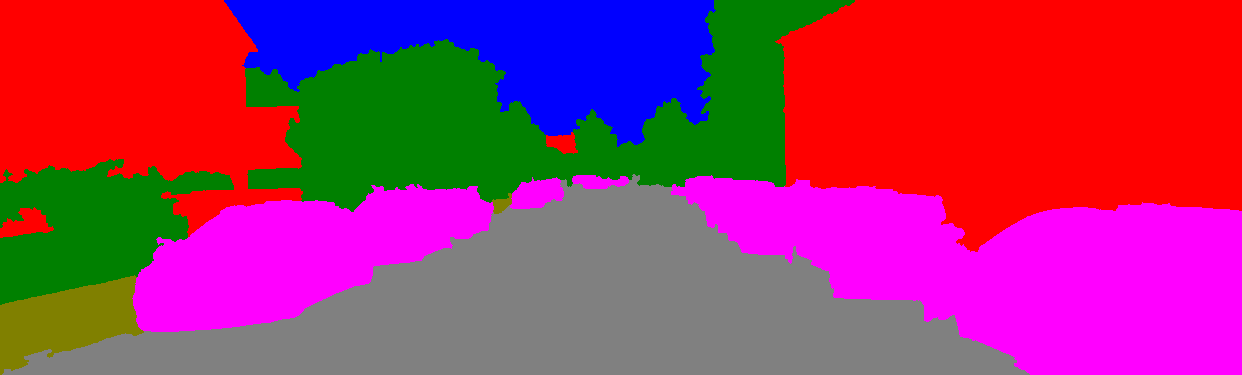
\includegraphics[width=0.4\textwidth]{images/sem310.png}}
    }
    \mbox{%
    \subfigure{\label{teste1d}%
      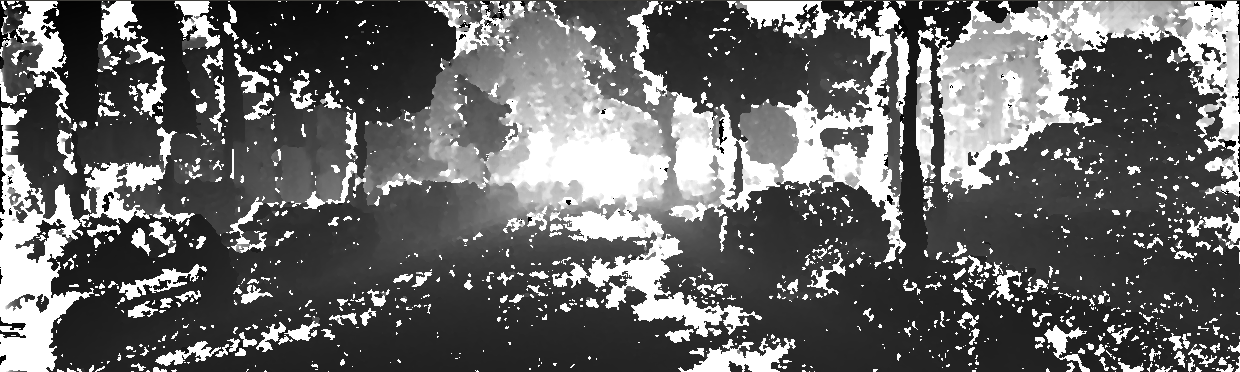
\includegraphics[width=0.4\textwidth]{images/disp35.png}}\qquad
    \subfigure{\label{teste2d}%
      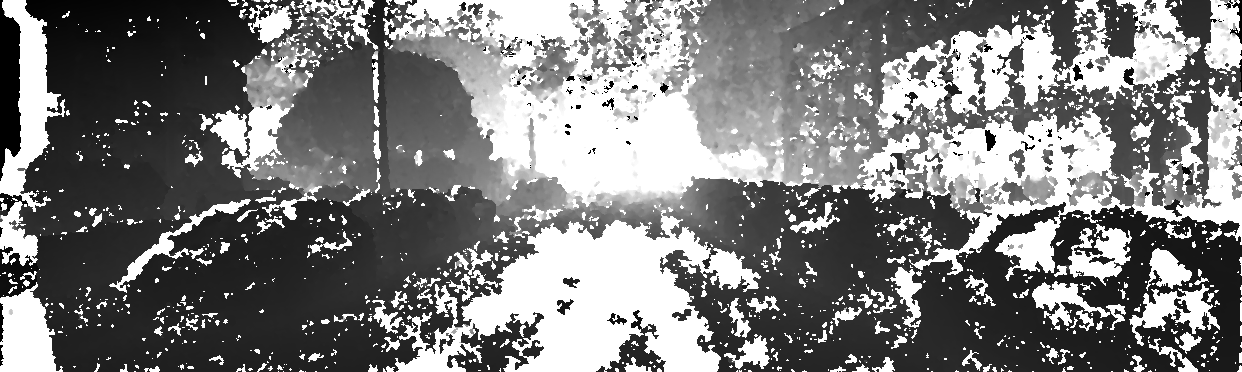
\includegraphics[width=0.4\textwidth]{images/disp310.png}}
    }
    \mbox{%
    \subfigure{\label{teste1d}%
      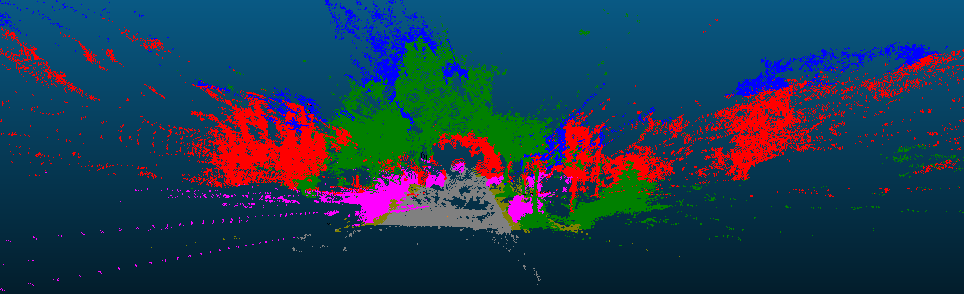
\includegraphics[width=0.4\textwidth]{images/color35.png}}\qquad
    \subfigure{\label{teste2d}%
      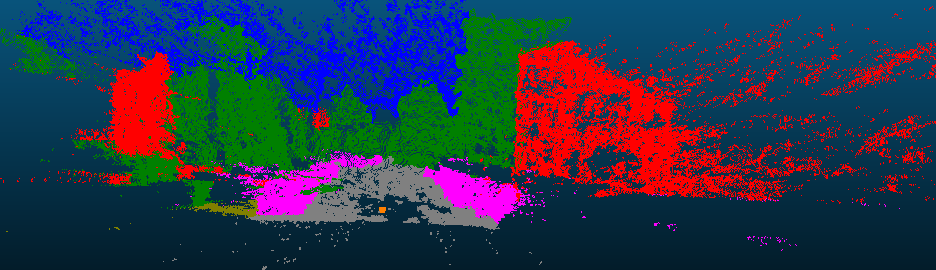
\includegraphics[width=0.4\textwidth]{images/color310.png}}
    }
    \mbox{%
    \subfigure{\label{teste1d}%
      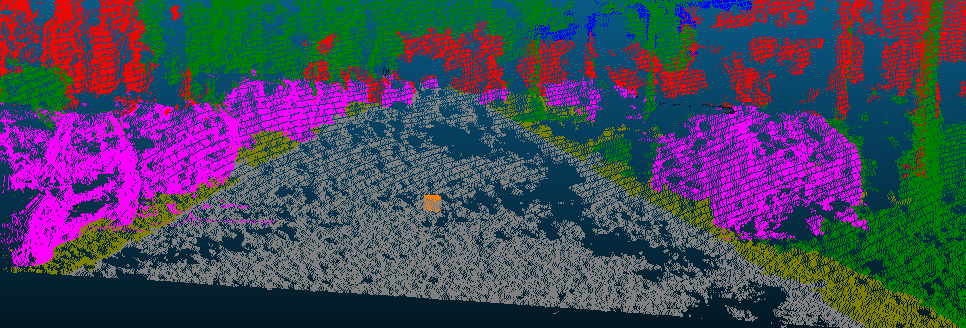
\includegraphics[width=0.4\textwidth]{images/zoom35.png}}\qquad
    \subfigure{\label{teste2d}%
      \includegraphics[width=0.4\textwidth]{images/zoom310.png}}
    }
    \legend{Source: Authors of this study.}
\end{figure}
    
    In addition, it was noted that the Cartesian plane used follows the pattern shown in \autoref{fig:CartesianPlane}, where the camera located in the car is taken as the axis (0,0,0).

    \begin{figure}[H]
    \caption{
        \label{fig:CartesianPlane}
        Cartesian plane used in Point Cloud
        }
        \begin{center}
        \includegraphics[scale=1]{images/eixos.png}
        \end{center}
        \legend{Source: Authors of this study.}
    \end{figure}
    
    The mass centers of the two cars analyzed in the test of \autoref{Teste1Center} can be seen in \autoref{Table:Center1} while that of the test of \autoref{Teste1Center} can be seen in \autoref{Table:Center2} and them exemplified how lower these numbers are.
    
    \begin{table}[H]
    \centering
    \caption{X, y, and z axis coordinates of the test of \autoref{Teste1Center}}
    %\vspace{0.2cm}
    \label{Table:Center1}
    \begin{tabular}{r|lll}
    Teste & X-axis & Y-axis & Z-axis \\ 
    \hline                               
    Car 1 & -0.417017   & 0.0258149 & 0.628768 \\
    Car 2 & -0.427101   & 0.0166311 & 0.78519       
     
    \end{tabular}
    \end{table}

    \begin{table}[H]
    \centering
    \caption{X, y, and z axis coordinates of the test of \autoref{Teste2Center}}
    %\vspace{0.5cm}
    \label{Table:Center2}
    \begin{tabular}{r|lll}
    Teste & X-axis & Y-axis & Z-axis \\ 
    \hline                              
    Street 1 & -0.193943   & 0.0495407 & 0.698221 \\
    Street 2 & -0.153351   & 0.0435096 & 0.700954   
     
    \end{tabular}
    \end{table}

    Therefore, one has to challenge the construction of a metric to convert these small coordinate values ​​into useful values ​​in the 3D environment
    
\subsection{Errors analysis.}

    This system has well-defined stages for its development and this has the benefit of the facility in identifying errors before are propagated.
    
    The first stage is camera calibration. The calibration itself can carry various types of errors and, according to \cite{ErrosCalibracao}, these can be categorized as:
    
    \begin{itemize}
    \item Gross Errors: This error is caused by the inability or neglect of the measurer;
    \item Accidental (or random) mistakes: These errors are caused by the imperfection of our senses, atmospheric irregularities and inevitable minor errors in instrument construction;
    \item Systematic errors: Errors caused by non-conforming measures (such as dilated timing, bent bolt and dumbbell post);
    \item Rounding Errors: Typically caused by the use of numbers with a few decimal places.

\end{itemize}

    It is possible that the system is subject to all these errors, although there are efforts to avoid them, such as using as many decimals as possible, both in calibration and in subsequent steps.
    
    In the following steps of calculating the disparity map it is possible to highlight some reasons for the difficulties already reported, such as low-contrast image regions. This problem impacted the results shown in order to create holes in the disparity map generating a noise that propagated to the end of the flow and hampered the faithful acquisition of the features.
    
    Another factor that contributed to the difficulty in generating a plausible graphical environment was the fact that the Point Cloud is generated by small coordinates. These values were between 5 and -5, with six decimal places in each coordinate. These low numbers contributed to the propagation of the error, since any small rounding in the center of mass calculation or in the bounding box will already result in very disparate values when passed to the 3D environment.

\section{3D environment}
    
    The 3D environment is expected to receive as input the identified entities, their information (position, direction and size), and standard 3D Model  that better represent it, and as output display an approximate scene from what was identified by the computer vision algorithm. A general flow of expected input and output is shown in \autoref{fig:3D-representation-flow}.
    
    \begin{figure}[H]
    \caption{
        \label{fig:3D-representation-flow}
            3D representation flow
        }
        \begin{center}
        \includegraphics[scale=0.65]{images/3D_representation.png}
        \end{center}
        \legend{Source: Authors of this study.}
    \end{figure}
    
    It was decided to develop the 3D environment system using C++ in conjunction with the graphical framework OpenGL, as it was considered the possibility of resource constraints, such as usage of CPU \& Memory and processing time. The system uses the OpenGL Shading Language (GLSL) for manipulation of VertexShaders and FragmentShaders. These choices, aside from the previous points, were based on authors' affinity with languages and frameworks while also allowing for more control on the program execution and better comprehension of the graphics pipeline of modern frameworks since both options are in a considerable low abstraction layer.
    
\subsection{Software Architecture}
    
    Following the Data-Oriented Design concept presented in the Literature Review chapter, an Entity Component System was projected as shown in \autoref{fig:kagami-simplified-diagram}.
    
    \begin{figure}[H]
        \caption{
        \label{fig:kagami-simplified-diagram}
            3D environment simplified diagram
        }
        \begin{center}
        \includegraphics[scale=0.65]{images/kagami-simplified-diagram.png}
        \end{center}
        \legend{Source: Authors of this study.}
    \end{figure}
    
    The control class of the system can be identified in \autoref{fig:kagami-simplified-diagram} as the class Engine, it has methods to initialize the main loop of the software and contains calls for defined Systems. Aside from the importance of the class Engine, three other classes deserve a more thorough description:
    
    \begin{itemize}
        \item Entity
        
        Represents the objects of the program, it maps the components existent in the software such as objects in a scene.
        
        \item Component
        
        Represents the differentiation of data stored in the program, it is mapped by the Entity class and all it's processing is dependent and executed by System classes. 
        
        \item Systems
        
        Are the real operators of the engine, it runs a defined data transformation (like defined on RendererSystem) on all the correct data of the program in a sequential manner). For example, RendererSystem conducts data transformation of all the entities which contains the Component's inherited class "RenderableComponent".
        
    \end{itemize}

\subsection{Display Evaluation}

    The 3D environment is capable of loading objects with information provided by the Cloud Analysis system. The input is the position coordinates (\(x\), \(y\), \(z\)), its orientation (\(theta\)), its size (Width, Length, Height) and semantic class (Car: 1, Street: 2).

    To evaluate the functionality of the 3D environment, a scene with one car was selected as shown in \autoref{fig:selected_test_visualization}. 
    
    \begin{figure}[H]
          \centering
          \caption{
        Scene for visualization test}
          \label{fig:selected_test_visualization}
            \subfigure{\label{testevisualization1a}%
              \includegraphics[width=0.4\linewidth]{images/right415.png}}\\
            \subfigure{\label{testevisualization1b}%
              \includegraphics[width=0.4\linewidth]{images/left415.png}}\\
            \subfigure{\label{testevisualization1c}%
              \includegraphics[width=0.4\linewidth]{images/sem415.png}}\\
            \subfigure{\label{testevisualization1d}%
              \includegraphics[width=0.4\linewidth]{images/color415.png}}\\
            \subfigure{\label{testevisualization1e}%
              \includegraphics[width=0.4\linewidth]{images/result_pointcloud.png}}\\
            \legend{Source: Authors of this study.}
    \end{figure}
    
    Thus, using \autoref{fig:selected_test_visualization} the point cloud as reference (bottom image), a baseline 3D environment input was crafted using \cite{giovaniThesis} semantic colors as shown in \autoref{fig:crafted_baseline}.
    
    \begin{figure}[H]
          \centering
          \caption{
        Crafted baseline}
          \label{fig:crafted_baseline}
            \subfigure{\label{crafted_baselinea}%
              \includegraphics[width=0.7\linewidth]{images/sem415.png}}\\
            \subfigure{\label{crafted_baselineb}%
              \includegraphics[width=0.7\linewidth]{images/result_pointcloud.png}}\\
            \subfigure{\label{crafted_baselinec}%
              \includegraphics[width=0.7\linewidth]{images/result_tailored.png}}\\
            \legend{Source: Authors of this study.}
    \end{figure}
    
    To evaluate the performance of the first system feature extractors, \autoref{fig:feature_extractors_visualization} shows:
    
    \begin{itemize}
        \item Top-Left: Crafted baseline;
        \item Top-Right: Simplified crafted baseline showing only car and street;
        \item Bottom-Left: Center of mass feature;
        \item Bottom-Right: Variance feature.
    \end{itemize}
    
        \begin{figure}[H]
          \centering
          \caption{
        Feature extractors comparison}
          \label{fig:feature_extractors_visualization}
          \mbox{%
            \subfigure{\label{fig:Ng1}%
              \includegraphics[width=0.5\linewidth]{images/result_tailored.png}}
            \subfigure{\label{fig:Ng2}%
              \includegraphics[width=0.5\linewidth]{images/result_tailored_simplified.png}}
            }
            \mbox{%
            \subfigure{\label{fig:Ng3}%
              \includegraphics[width=0.5\linewidth]{images/result_centerofmass.png}}
            \subfigure{\label{fig:Ng4}%
              \includegraphics[width=0.5\linewidth]{images/result_variance.png}}
            }
            \legend{Source: Authors of this study.}
        \end{figure}
        
    Comparing feature extractors, it's possible to say that the center of mass method showed better results in relation to position but bad due to it's smaller scale in relation to the baseline, while the variance method have better coverage of the baseline car. When considering a user point of view for an interface, the variance method performed better for car representation. 
    
    Since the current Cloud Analysis doesn't provide more than one entity for one semantic class, the street object is on the comparison picture for spatial reference.
    
    Case scenarios are limited due to the constraint of one type of semantic class. However, it's possible to confirm the visualization functionality of the 3D environment.